%%============================================================================%%
%% JEPA-Based Representation Learning for High-DoF Metasurface Inverse Design
%% Structure follows the author's outline. All numbers were produced by the
%% repository's own runs; dataset statistics were measured from the split files.
%% References are peer-reviewed venues only.
%%============================================================================%%
\documentclass[pdflatex,oneside,sn-mathphys-num]{sn-jnl}

\usepackage{graphicx}
\usepackage{float}
\usepackage{multirow}
\usepackage{amsmath,amssymb,amsfonts}
\usepackage{amsthm}
\usepackage{mathrsfs}
\usepackage[title]{appendix}
\usepackage{xcolor}
\usepackage{textcomp}
\usepackage{manyfoot}
\usepackage{booktabs}
\geometry{twoside=false, left=22mm, right=22mm, top=22mm, bottom=24mm}
\AtBeginDocument{\geometry{twoside=false, left=22mm, right=22mm, top=22mm, bottom=24mm}%
\csname @twosidefalse\endcsname
\setlength{\oddsidemargin}{-9.9pt}
\setlength{\evensidemargin}{-9.9pt}
\setlength{\textwidth}{455.2pt}
\typeout{PGMARGINS odd=\the\oddsidemargin even=\the\evensidemargin width=\the\textwidth twoside=\if@twoside yes\else no\fi}}

\theoremstyle{thmstyleone}
\newtheorem{theorem}{Theorem}
\theoremstyle{thmstyletwo}
\newtheorem{example}{Example}
\theoremstyle{thmstylethree}
\newtheorem{definition}{Definition}

\raggedbottom

\begin{document}

\title[Article Title]{JEPA-Based Representation Learning for High-Degree-of-Freedom Metasurface Inverse Design}

\author[1]{\fnm{Tejas P.} \sur{Biradar}}\email{23bec129@iiitdmj.ac.in}
\equalcont{These authors contributed equally to this work.}

\author[1]{\fnm{Akash} \sur{Kesav}}\email{23bsm006@iiitdmj.ac.in}
\equalcont{These authors contributed equally to this work.}

\author*[1]{\fnm{Ponappa} \sur{K.}}\email{kponappa@iiitdmj.ac.in}

\affil*[1]{\orgname{PDPM Indian Institute of Information Technology, Design and Manufacturing, Jabalpur,
482005, Madhya Pradesh, India.}}

\abstract{
Inverse design of metasurfaces is difficult for a reason that is usually stated too
loosely: the target spectrum does not determine a unique geometry, so a model trained to
minimise an output loss can satisfy that loss without ever using the spectrum. We address
this directly and make the conditioning non-negotiable, at three levels. The design is
factorised into a single-channel $64\times64$ occupancy map and three explicit physical
parameters with known/unknown flags, so the geometry and the parameters can be masked
independently and the model is never handed a parameter disguised as a pixel. The
spectrum enters through a frozen released encoder and drives two separate pathways, a
token-level goal that the predictor attends to and a global physics condition applied as a
per-block FiLM modulation; a second copy of that modulation is frozen on the target
encoder, so the objective cannot make the target spectrum-free in order to reduce the
loss. Finally, the released corpus is exactly invariant under the four-fold mirror group
(verified over all 174{,}883 patterns), so the occupancy decoder predicts one
$32\times32$ quadrant and mirrors it, which makes every generated design admissible by
construction. The result is a deterministic, goal-constrained generative model rather
than a regressor: $11.6$M trainable parameters, $3.2\times$ fewer than the released
MetaDiT-S baseline, with a held-out test error of $0.0524\pm0.0014$ MAE against $0.0801$.
On a paired real-versus-deranged-goal test, which no output-averaging model can pass by
accident, the true goal wins on $99.3\%$ of pure-inverse samples, $97.1\%$ with partial
geometry and $93.0\%$ in retrofit.
}

\maketitle

\section{Introduction}\label{sec1}

A metasurface is a planar array of sub-wavelength scatterers whose optical response is
set by geometry. Designing one means choosing a unit-cell shape and a few physical
parameters so that the transmitted spectrum matches a target. Two properties make this
difficult. The forward map is expensive: one full-wave simulation at fabrication-grade
resolution costs minutes to hours, so a solver cannot sit inside an optimisation loop
that evaluates thousands of candidates. And the inverse map is one-to-many: distinct
geometries produce nearly identical spectra, so a point estimate is a choice among
admissible answers rather than a recovery.

The standard remedy is to amortise the solver into a learned model and invert that.
Existing routes regress the geometry directly, generate it from a conditional
distribution, or retrieve it from a library~\cite{empowering,roadmap,revisit}. All three
share a weakness that is easy to miss: a network trained only to minimise an output
loss may satisfy that loss without using the conditioning signal, because the training
data alone supply enough structure to fit the marginal.

This paper treats inverse design as representation learning. We adapt a
joint-embedding predictive architecture (JEPA), in which a student predicts the latent
representation of a masked region from visible context while an
exponential-moving-average teacher supplies the target~\cite{ijepa}. Applied here, the
occupancy encoder sees a partially masked occupancy map and nothing else, so the
geometry representation is built without the spectrum; the spectrum then conditions
latent completion through two pathways, sixteen goal tokens entering the fusion stage
and a global physics vector modulating every predictor block. The teacher sees the
complete geometry and is additionally modulated by the true spectrum, so matching it
requires the goal to have entered the prediction.

Our model differs from a textbook JEPA in three ways. The design is factorised into an
occupancy map, three flagged parameters and the spectrum, with the three-channel
broadcast tensor assembled only at the surrogate boundary, so spatial and parameter
masking stay independent. The spectrum enters through a frozen released encoder that
drives both a global FiLM path~\cite{film} and sixteen attention tokens, and the FiLM that acts on
the target is frozen so the conditioning cannot be optimised away. Finally, the
occupancy decoder predicts a single quadrant and mirrors it, which is exact for this
corpus and makes every output admissible.

\section{Background and Related Work}\label{sec2}

Inverse design is the problem of finding an input to a physical system that produces a
prescribed output, when the forward map is known but expensive and the inverse map is
not unique. Classical treatments alternate between a solver and an optimiser, which is
accurate but slow, or build a differentiable approximation of the forward map and
descend through it. Learned approaches instead amortise the solver into a model that is
evaluated once per query, and differ in what that model is trained to output: a point
estimate of the design~\cite{tandem,structuralcolor}, a distribution over
designs~\cite{genmodel}, or a ranking over a fixed library~\cite{moclip}. Point
estimates inherit the ambiguity of the inverse map and tend to return an average of
competing answers. Distributions avoid that but need sampling and a noise schedule, and
their conditioning can be underused because the training objective is satisfied by the
data marginal alone. Retrieval is exact inside the library and cannot leave it. Surveys
across photonics make the same observation from the applied side: accuracy is limited
by the representation a model learns, not by its capacity, and a network that is never
forced to use its conditioning will ignore it~\cite{empowering,ailarge,deepmetasurfaces,largescale}.

Joint-embedding predictive architectures take a different route to the same goal. Instead
of reconstructing inputs, they predict the representation of a masked region from the
visible context, with the target produced by an exponential-moving-average copy of the
encoder~\cite{ijepa}. Since the loss is computed in representation space, nuisance
detail is not reconstructed, and since the target is learned rather than fixed, a
one-to-many map need not collapse to a single label. Masked autoencoding is the closest
relative but reconstructs pixels~\cite{mae}, which for a design problem rewards copying
whatever structure is already visible. The failure mode shared by all joint-embedding
methods is collapse, prevented by constraining the embedding statistics: VICReg combines
an invariance term with a variance hinge and a covariance term~\cite{vicreg}. Conditioning in such
architectures is usually implemented as feature-wise linear modulation~\cite{film},
which in transformer form becomes adaptive layer normalisation with zero-initialised
gates. We use all of these, but assign them distinct jobs: FiLM carries the
global condition at every block, goal tokens carry fine structure through attention, and
a frozen modulation on the target makes the conditioning impossible to remove.

Metasurfaces are the setting in which these ideas are tested here. A metasurface is a
planar array of sub-wavelength scatterers whose response is set by geometry, so the
design is an image and the forward map is an electromagnetic solve. The field has
adopted learned inverse design quickly, first with tandem
networks~\cite{tandem,structuralcolor}, then with generative
models~\cite{genmodel}, and most recently with large-scale pipelines in which the
bottleneck is the cost of evaluating candidates rather than the network
itself~\cite{largescale,vr,roadmap,revisit}. Two properties of the domain shape the
design space: the parameters that matter are few and physically interpretable, and the
solver is accurate but far too slow to sit inside a training loop, which is why a frozen
surrogate is standard. The circularity that follows, where a model is scored by the same
surrogate it was optimised through, is usually handled by reporting an independent
metric alongside, and we do the same.

MetaDiT is the closest prior work and the source of our data, split and forward
surrogate~\cite{metadit}. It formulates inverse design as conditional generation: a
diffusion transformer~\cite{dit} over a three-channel broadcast tensor
$(G\odot r/5,\ G\odot h,\ l/3)$, where $G\in\{0,1\}^{64\times64}$ is the binary occupancy map and $\odot$ is the
elementwise product. The map is what confines the first two channels to the material:
they hold a constant value on occupied pixels and are exactly zero elsewhere, whereas
the third channel is constant over the whole cell.
Trained with a denoising
objective~\cite{ddpm} and conditioned on the target spectrum, reporting a mean absolute
spectral error of $0.0801$ and an accumulated error of $48.25$ on the released test
split. Its generator produces a $32\times32$ quadrant that is thresholded and mirrored
to $64\times64$, so its output is symmetric by construction. We keep the data, the split
and the surrogate unchanged so that numbers are comparable, and change three things: the
design is factorised into occupancy and explicit parameters instead of a broadcast
tensor; the generator is a deterministic JEPA instead of a diffusion process; and the
spectral conditioning is made structurally non-nullifiable. The first change addresses a
specific weakness of the broadcast form, in which $l/3$ is constant over the cell, so
the lattice constant is readable from a single pixel and a masked-region objective is
partly answerable without the region's neighbours. The second and third address the
observation above: a side condition with no term penalising its neglect is easy to
ignore, and the evaluation protocol of Section~\ref{sec4} is built to detect exactly
that failure by comparing the true goal against a deranged goal from the same batch.

\section{Our Model}\label{sec3}

Figure~\ref{fig:arch} gives the full data flow, and Figure~\ref{fig:blocks} opens the
three stages that are otherwise drawn as single boxes.

\begin{figure}[h]
\centering
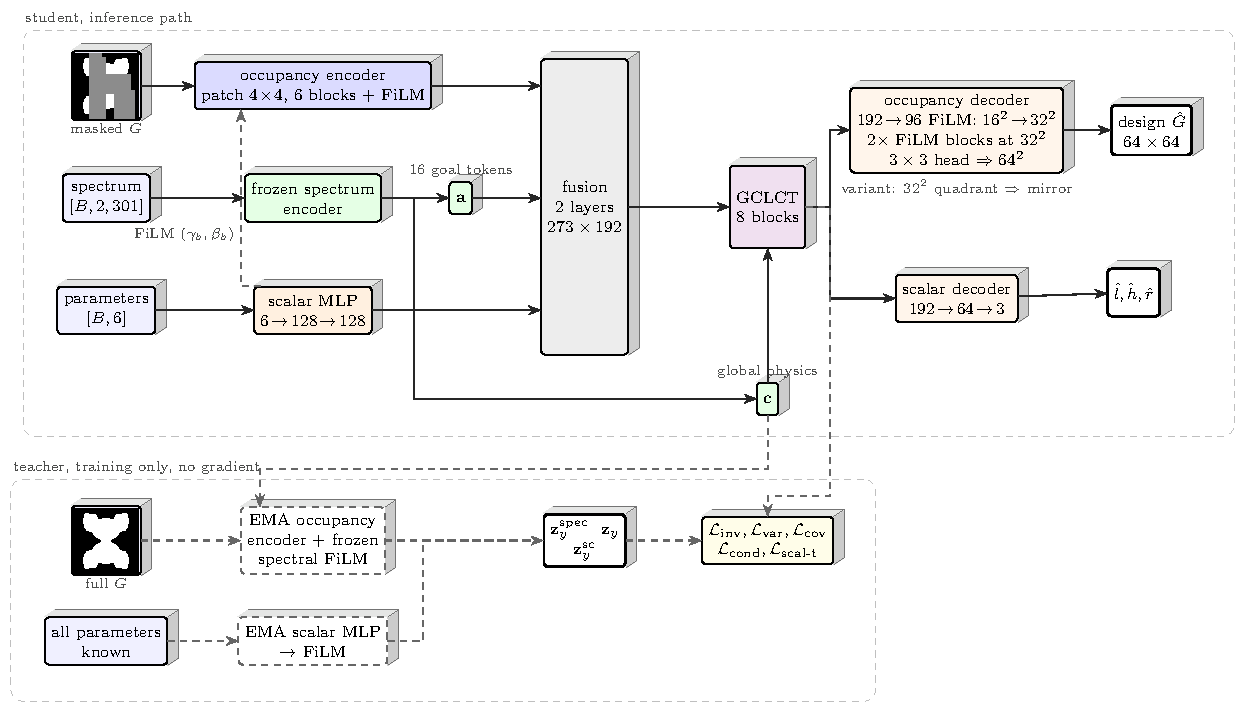
\includegraphics[width=\textwidth]{figs/architecture.pdf}
\caption{Architecture. The student band (solid arrows) is the inference path. The teacher
band (dashed) mirrors it: an exponential-moving-average copy of the occupancy encoder,
modulated by a frozen FiLM driven by $\mathbf{c}$, produces the spectrum-conditioned target,
and an EMA copy of the scalar branch produces the target FiLM and the scalar latent. The
teacher never receives gradients. The student input panel is a real held-out sample with the masked tokens drawn in
grey and the visible material in white, so what the encoder hides is visible in the
figure itself; the teacher receives the complete pattern.}
\label{fig:arch}
\end{figure}

\subsection{Dataset and semantic factorisation}

We use the released MetaDiT corpus~\cite{metadit}, unchanged. Each sample contains a
$64\times64$ binary occupancy map $G$, three scalar parameters, lattice constant $l$,
meta-atom thickness $h$ and meta-atom refractive index $r$, and the complex transmission spectrum
on 301 frequency samples. Measured over the corpus, $l\in[2.5,3.0]$,
$h\in[0.5,1.0]$ and $r\in[3.5,5.0]$, with means $2.750$, $0.828$ and $4.489$. The
occupancy fraction averages $0.421$ and spans $0.028$ to $0.632$ per sample, so the
occupied class is neither rare nor dominant and pixel accuracy would be a misleading
metric. The released split is used as published: 139{,}906 training, 17{,}488
validation and 17{,}489 test samples.

The spectrum is kept complex, as two real channels of 301 samples each, rather
than reduced to an amplitude. Amplitude alone loses the phase relation between
frequencies, and two designs that differ only in resonant phase can have nearly
identical amplitude curves while producing different transmitted fields. Keeping
both channels also matches the interface of the released encoder, which was trained
on this representation; converting it would put our targets in a different domain
from the surrogate's training data.

The corpus stores each design in the broadcast form
\begin{equation}
\mathbf{x}_0 = G\odot(r/5),\qquad
\mathbf{x}_1 = G\odot h,\qquad
\mathbf{x}_2 = l/3,
\end{equation}
where $G$ is the binary occupancy map defined above and $\odot$ is the element-wise
product. The operation is a mask, not a channel-wise transform: at every pixel inside the
material the first channel holds $r/5$ and the second holds $h$, and at every pixel outside
it both hold exactly zero, while the third channel carries the same value $l/3$ at every
pixel of the cell. This is convenient for the surrogate and destructive for learning: $l$ is readable
from any pixel, and a masked-region objective over the tensor is partly answerable without
the region's neighbours. We therefore factorise every sample before it reaches the network,
\begin{equation}
(G, l, h, r) \;\longleftrightarrow\;
\big(G\in\{0,1\}^{1\times64\times64},\ (l,h,r)\in\mathbb{R}^3\big),
\label{eq:fact}
\end{equation}
and reassemble the broadcast tensor only when the surrogate has to be called.

The practical consequence is that the two mask families become orthogonal
controls. A spatial mask withholds geometry while leaving the parameters intact;
a scalar mask withholds the parameters while leaving the geometry intact; and the
two can be combined at arbitrary rates. On the broadcast tensor this separation is
impossible, because a parameter is encoded as a region of the tensor itself, so
masking a block of pixels also destroys part of the parameter signal and the two
effects cannot be attributed. Because
the transformation is exact in both directions, masking can be applied to the occupancy
and to the parameters as two independent operations, which is what makes the three
regimes of Section~\ref{sec4} well defined.

\subsection{Notation}

The figures and the rest of this section use the following shorthand. LN is layer
normalisation, applied per token across feature dimensions. MHSA is multi-head
self-attention, which lets tokens exchange information through several attention heads in
parallel. MLP is the feed-forward block applied after attention. FiLM is feature-wise
linear modulation, which rescales and shifts feature channels with coefficients computed
from a condition. EMA is an exponential moving average of weights, used for the teacher.
Residual connections are written as
\begin{equation}
\mathbf{x}_{\mathrm{out}} = \mathbf{x} + f(\mathrm{LN}(\mathbf{x})),
\end{equation}
and every sub-layer in the model follows this form.

Two FiLM placements must not be confused, because they sit at different points in the
network. In the predictor, every block applies the spectrum condition three times, once
before each sub-layer, in the order LN, FiLM, self-attention, residual; LN, FiLM,
cross-attention, residual; LN, FiLM, MLP, residual. In the occupancy encoder, the scalar
condition is applied once per block, after that block's residual output. The two use the
same mechanism but different geometry.

\subsection{Encoder}

The encoder is deliberately split into three branches with different jobs: the scalar
branch turns physical parameters into a modulation, the occupancy branch turns the cell
into spatial tokens, and the spectrum branch turns the target into a condition. They
meet only at the fusion stage.

\subsubsection{Scalar branch}
The branch receives six numbers per sample,
\begin{equation}
\mathbf{s} = [\, l,\ k_l,\ h,\ k_h,\ r,\ k_r \,],
\end{equation}
where $k_\bullet\in\{0,1\}$ states whether that parameter is observed. Unknown values are set to zero and the flag carries the
distinction between ``absent'' and ``equal to zero'', so the encoder never has to infer
missingness from a magnitude. A two-layer perceptron with GELU activations,
\begin{equation}
6 \;\longrightarrow\; 128 \;\longrightarrow\; 128,
\end{equation}
produces two outputs.

The first is a set of FiLM coefficients, one pair per occupancy-encoder block,
\begin{equation}
(\gamma_b,\ \beta_b) \;\in\; \mathbb{R}^{192}\times\mathbb{R}^{192},
\qquad b = 1,\dots,6,
\end{equation}
applied as
\begin{equation}
\mathbf{x} \;\mapsto\; \gamma_b\odot\mathbf{x}+\beta_b .
\end{equation}

One pair per block, rather than one pair shared across depth, is what lets the
parameters act differently at different scales of abstraction: an early block sees
local patch statistics where the lattice constant matters most, while a late block
sees a global summary where thickness and refractive index dominate. The modulation is applied
after the block's residual sum, not inside the attention, so the attention weights
themselves remain a function of the geometry alone and the parameter path stays
separable for later inspection. The head is initialised with zero
weights and with $\gamma$ biased to one, so the modulation is the identity at step zero
and the network is free to leave it there. The second output is a $192$-dimensional
summary token that enters the fusion stage; it is trained by its own read-out term,
which gives the branch a gradient path that does not pass through the predictor, a
detail that matters because otherwise the parameters reach the model only through a
deep and easily-saturated route.

\subsubsection{Occupancy branch}
The occupancy encoder is a vision transformer~\cite{vit} over the cell. A convolution
with kernel and stride four maps each non-overlapping $4\times4$ patch to a
$192$-dimensional vector; the $64\times64$ grid becomes a $16\times16$ grid of tokens,
and flattening gives
\begin{equation}
G\in\{0,1\}^{1\times64\times64}
\;\longrightarrow\;\mathbf{z}_x\in\mathbb{R}^{256\times192},
\end{equation}
that is, $256$ tokens of width $192$. Masking is applied at token granularity: a token
whose $4\times4$ block is masked is replaced by a learned mask token before the
positional embedding is added, so the encoder never sees the hidden pixels in any form,
not even indirectly through a patch statistic.

The ordering matters: the mask token is substituted before the positional
embedding is added, so a masked position still carries its location but nothing
about its content. Adding the embedding first and masking afterwards would leak
the patch through the position-dependent offset, which is the same class of leak
that the broadcast tensor introduces for the lattice constant. The mask token is a
single learned vector shared by all masked positions, so the decoder cannot tell
how many neighbours a given masked token had.

Six pre-norm transformer blocks follow, each with six heads and an MLP ratio of four.
Every block applies self-attention, a residual sum, an MLP, a second residual sum, and
then the scalar FiLM transform. Layer normalisation is used without learned affine
parameters so that all modulation enters through FiLM, which keeps the two conditioning
paths separable. The occupancy encoder is spectrum-agnostic by construction: the spectrum reaches the
model only downstream, as goal tokens in the fusion stage and as the global condition on
the predictor, never as an input to this encoder.

\subsubsection{Spectrum branch}
The spectrum is processed by the released MetaDiT spectrum encoder~\cite{metadit},
which is frozen. It maps the $2\times301$ complex response to $301$ tokens of width
$256$. Two read-outs are taken. The mean token, projected to $384$ dimensions, gives
the global condition $\mathbf{c}$, which summarises the overall electromagnetic
behaviour the design must achieve. Sixteen learned queries cross-attend to the frequency
tokens and give
\begin{equation}
\mathbf{a} \in \mathbb{R}^{16\times384},
\end{equation}
where each query specialises to a
different aspect of the response, so fine structure survives instead of being averaged
into a single vector. Both read-outs are projected to width $192$ downstream.

The division of labour between the two read-outs is deliberate. The global vector
answers ``what should this design do overall'', which is enough to set the family
of the response but not to place a narrow resonance. The sixteen queries answer
"which parts of the curve matter'', and because they enter as attention tokens the
predictor can attend to one of them and ignore the rest. A single pooled vector
forces every frequency to contribute, which averages away exactly the narrow
features that distinguish two otherwise similar targets. Freezing
the encoder is deliberate: it is a released reference model, and allowing it to move
would let the objective reshape the very representation the surrogate was trained
against.

\subsection{Fusion transformer and GCLCT}

The three branches are concatenated after projection to a common width,
\begin{equation}
\mathbf{f}=\mathrm{Fusion}\big([\mathbf{z}_x;\ \mathbf{a};\ \mathbf{s}_\Sigma\big])
\in\mathbb{R}^{273\times192},
\end{equation}
with $256$ occupancy tokens, $16$ goal tokens and one scalar-summary token. The fusion
module is a two-layer transformer; its role is to let goal tokens exchange information
with the geometry before prediction while keeping the goal an attributable block of the
context.

Three details matter for what follows. The sixteen goal tokens are projected from 384 to
192 dimensions by a single linear map before concatenation, while the occupancy tokens
arrive already at width 192 from the encoder, so the concatenation is dimensionally
uniform but semantically asymmetric: the geometry block carries spatial position through
its own positional embedding, whereas the goal and summary blocks carry none, because a
goal token has no location. The fusion stack is deliberately shallow, two blocks, because
its job is not to reason about the design but to let the goal tokens read enough geometry
to become useful context. Deeper fusion was not needed: the heavy reasoning happens in
the predictor, and a deeper fusion stack would compete with it for capacity while adding
attention cost over the longest sequence in the model.

The reason the goal is split into two pathways at all is that one mechanism cannot do both
jobs. A single pooled vector is a global statement about the response and is the right
input for a per-block affine modulation, but it cannot express which part of a curve
matters. A set of tokens can express that through attention, but as attention context it
acts only where the queries look. Carrying both means the spectrum shapes every block's
computation through FiLM while also being available as retrievable detail, and the two
paths fail differently: the global path can be ignored if its modulation learns to be the
identity, and the token path can be ignored if attention learns to look elsewhere. Neither
can be removed silently without the other showing it.

Prediction is performed by a Goal-Conditioned Latent Completion Transformer (GCLCT) of
depth eight. It consumes $257$ queries, one per cell token plus a single learned
scalar query, and attends over the $273$ fused tokens. Each block applies an
affine-free layer norm, a FiLM modulation from $\mathbf{c}$, self-attention among the
queries, a second normalised FiLM and a cross-attention whose keys and values are the
fused tokens, and a third normalised FiLM and an MLP, each with a residual sum. The
FiLM generator is zero-initialised~\cite{dit}, so each block begins as the identity and
must learn to use the condition; with eight blocks the condition acts at eight
different depths rather than once.

The attention cost is modest because the query set is short: cross-attention is
over $257\times273$ pairs rather than over the square of the context, and the
context itself is only $273$ tokens. This is what allows the predictor to be the
largest module in the model, eight blocks, $6.6$M parameters, more than half of
the trainable budget, without making inference expensive. The $273$ fused tokens
are recomputed once per sample, and the eight predictor blocks then operate on a
fixed-size query set, so runtime scales with depth rather than with cell area.

The output splits into $256$ predicted geometry latents $\hat{\mathbf{z}}$ and one
scalar latent $\hat{\mathbf{s}}_\Sigma$.

Three properties of this stack are worth stating explicitly. First, the condition enters
through a projection from 384 to 192 dimensions, one per block, and every projection is
zero-initialised together with its gate, so at step zero each block is exactly the
identity and the model begins as a plain latent-completion transformer; the conditioning
is learned, not imposed. Second, the queries are not the context: the $273$ fused tokens
are keys and values, while the $257$ queries are a fixed-size set that is rewritten at
every block. This is what keeps cost independent of cell size once the context exists, and
it is why the predictor can hold more than half of the trainable parameters without
dominating inference time. Third, the scalar query is the only query without a spatial
position, and it is the one that becomes the scalar prediction; putting it in the same
attention stack means the parameters are inferred with the same evidence as the geometry
rather than by a separate head reading a pooled vector.
 The scalar latent is routed through a small
three-headed perceptron to $(l,h,r)$; its final bias is initialised to the dataset
means rather than to zero, because a zero output drives the frozen surrogate's
activation into a dead region and no gradient reaches the branch.

\begin{figure}[h]
\centering
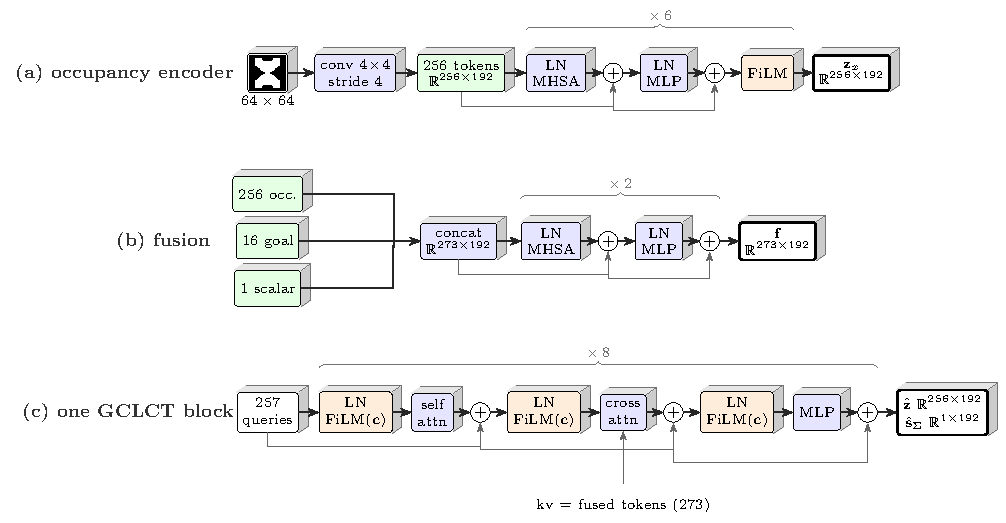
\includegraphics[width=\textwidth]{figs/blocks.pdf}
\caption{Internals of the three stages usually drawn as single boxes, flow left to right.
(a) Occupancy encoder: a $4\times4$ stride-4 convolution yields $256$ tokens of width $192$. LN is layer normalisation, MHSA multi-head self-attention, MLP a feed-forward block, $\oplus$ a residual sum;
six pre-norm blocks follow, each with a residual self-attention, a residual MLP and a FiLM
transform whose coefficients come from the scalar branch. (b) Fusion: the three token groups
are concatenated into $273$ tokens and passed through two transformer blocks. (c) One GCLCT
block: an affine-free layer norm and a FiLM modulation from the global spectrum condition
before each sub-layer, with a residual sum after every sub-layer; the middle sub-layer is the
cross-attention over the $273$ fused tokens. The stack repeats eight times.}
\label{fig:blocks}
\end{figure}

\subsection{Targets and the JEPA objective}

Two exponential-moving-average targets are maintained, one for the occupancy encoder
and one for the scalar encoder, with momentum ramped linearly from $0.996$ to $0.999$
over the run. Three quantities are produced under no gradient. The first is the plain
geometry target
\begin{equation}
\mathbf{z}_y = \mathrm{EMA}_{\mathrm{occ}}(G),
\end{equation}
computed on
the complete, unmasked cell and modulated by the scalar target. The second is a
spectrum-conditioned target, obtained by additionally modulating the target encoder
with a frozen FiLM whose coefficients come from $\mathbf{c}$; matching it requires the
goal, and freezing the modulation removes the objective's ability to make the target
spectrum-free again. The third is a scalar target $\mathbf{z}_y^{\mathrm{sc}}$ from the
EMA scalar branch, which forces the scalar path to carry its conditioning.

The exponential-moving-average target is what makes the objective non-degenerate.
If the target were the student's own output, the loss could be driven to zero by
collapsing both branches to a constant; the moving average makes the target lag,
so a collapsed student is always behind a slightly less collapsed teacher. The
momentum ramp matters for the same reason: too fast a teacher at the start gives a
target that moves with the student and the lag disappears, which is why the
momentum is tied to the total step count rather than fixed.

The prediction and both targets are projected by an MLP with batch normalisation owned
by the objective rather than by the model, and three VICReg terms are evaluated on the
masked tokens: an invariance mean-squared error, a variance hinge with threshold one,
and an off-diagonal covariance penalty~\cite{vicreg}. Keeping the projector in the
objective means the latent the encoder produces is the one that is regularised, not a
private projection of it.

\subsection{Losses}

The total objective is a weighted sum of nine terms,
\begin{equation}
\mathcal{L}=
\lambda_{\mathrm{inv}}\mathcal{L}_{\mathrm{inv}}
+\lambda_{\mathrm{var}}\mathcal{L}_{\mathrm{var}}
+\lambda_{\mathrm{cov}}\mathcal{L}_{\mathrm{cov}}
+\lambda_{\mathrm{sc}}\mathcal{L}_{\mathrm{sc}}
+\lambda_{\mathrm{occ}}\mathcal{L}_{\mathrm{occ}}
+\lambda_{\mathrm{ph}}\mathcal{L}_{\mathrm{ph}}
+\lambda_{\mathrm{sum}}\mathcal{L}_{\mathrm{sum}}
+\lambda_{\mathrm{cond}}\mathcal{L}_{\mathrm{cond}}
+\lambda_{\mathrm{st}}\mathcal{L}_{\mathrm{st}},
\label{eq:loss}
\end{equation}
defined in Table~\ref{tab:losses}. The first three act on projected masked latents, the
next two are direct supervision, and the last four tie the latent to the goal and to
the parameters.

\begin{table}[h]
\centering
\caption{Loss terms, weights and roles. $\mathcal{M}$ is the set of masked tokens and
$\mathcal{U}$ the set of unknown parameters.}\label{tab:losses}
\begin{tabular}{@{}llcl@{}}
\toprule
Term & Definition & Weight & Role \\
\midrule
$\mathcal{L}_{\mathrm{inv}}$ & MSE of projected prediction vs target on $\mathcal{M}$ & 25.0 & latent \\
$\mathcal{L}_{\mathrm{var}}$ & VICReg variance hinge, $\gamma=1$ & 25.0 & latent \\
$\mathcal{L}_{\mathrm{cov}}$ & VICReg off-diagonal covariance & 1.0 & latent \\
$\mathcal{L}_{\mathrm{sc}}$ & L1 on unknown parameters $\mathcal{U}$ & 1.0 & scalars \\
$\mathcal{L}_{\mathrm{occ}}$ & BCE on masked pixels & 1.0 & occupancy \\
$\mathcal{L}_{\mathrm{ph}}$ & smooth-L1 on std-normalised spectra & 3.32 & physics \\
$\mathcal{L}_{\mathrm{sum}}$ & L1 read-out of known parameters & 1.0 & scalars \\
$\mathcal{L}_{\mathrm{cond}}$ & $1-\cos$ to the spectrum-conditioned target & 0.5 & latent \\
$\mathcal{L}_{\mathrm{st}}$ & $1-\cos$ to the target scalar latent & 0.5 & latent \\
\botrule
\end{tabular}
\end{table}

The physics weight is the one coefficient that was measured rather than chosen. A
sweep over five values showed a non-monotone response: small weights
($0.03$ and $0.1$) made the pure-inverse error \emph{worse} than training with no
physics at all, while large weights improved it, and the best swept value was still
improving at the top of the range. The value used here is therefore a lower bound on
the optimum rather than a located maximum, and it is reported as such.

Two conventions govern reproduction. The physics term normalises prediction and target
by the per-sample standard deviation of the target spectrum, so a weakly responding
sample contributes proportionally, and the implementation refuses to normalise below a
floor of $10^{-3}$ rather than amplify noise. The same term is skipped on batches whose
goal was dropped for guidance, because there the target would be the condition that was
removed. Gradients reach the surrogate input but never its parameters: the surrogate is
frozen, excluded from the optimiser, and asserted to receive no gradient at every step.

Training uses AdamW~\cite{adamw} with a cosine schedule, batch size two with gradient
accumulation, and clipping at unit norm. Three curricula are applied. The masked
fraction is sampled per sample and its distribution is ramped from an easy to a hard
mixture over the first 3{,}000 steps. The physics weight is held at zero for 2{,}000
steps and ramped in over 3{,}000, so the representation forms before the surrogate
acts. The multi-target weights ramp in from step 1{,}000. The goal is dropped with
probability $0.1$ so the model learns both conditional and unconditional predictions.

\subsection{Symmetry prior in the decoder}

We verified the symmetry of the released data rather than assuming it: in all three
splits, every occupancy map is invariant under both reflections,
\begin{equation}
G \;=\; \mathrm{fliplr}(G) \;=\; \mathrm{flipud}(G)
\;=\; \mathrm{rot}_{180}(G),
\label{eq:sym}
\end{equation}
with no exceptions over 174{,}883 patterns. The data therefore occupy the fixed-point set
of the four-fold mirror group, and a decoder that predicts all $64\times64$ pixels spends
three quarters of its output degrees of freedom on directions the data never use.

We make the symmetry structural rather than learned. The occupancy decoder predicts one
$32\times32$ quadrant $Q$ and assembles the cell by reflection,
\begin{equation}
\hat{G} \;=\;
\begin{pmatrix}
Q & \mathrm{fliplr}(Q)\\[2pt]
\mathrm{flipud}(Q) & \mathrm{rot}_{180}(Q)
\end{pmatrix}
\in\{0,1\}^{64\times64},
\label{eq:quad}
\end{equation}
so Eq.~\eqref{eq:sym} holds for every output and every input. The quadrant comes from a
$192\!\to\!96$ FiLM block at $16\!\to\!32$ resolution, two resolution-preserving FiLM
blocks and a $3\times3$ head; the mirroring has no parameters and costs nothing at
inference.

This bounds the model as well as helping it. Because symmetry is a property of the
function class, an asymmetric design cannot be represented at all: on a corpus that
contained asymmetric unit cells the decoder would fail silently, returning a symmetric
approximation with a higher loss rather than an error. The constraint is therefore
justified by the measurement above and is not a general assumption about metasurfaces;
lifting it requires only using the unconstrained decoder variant, which we retain for that
purpose. Within this corpus it changes the admissibility of the output, not the spectral
accuracy, as Section~\ref{sec4} reports.

\subsection{Inference}

At inference the teacher and all losses are discarded. The student receives the target
spectrum, the visible part of the occupancy and the known parameters. It predicts the
masked latents, decodes the occupancy quadrant and the parameters, mirrors the quadrant,
restores the visible pixels exactly, substitutes known parameters with their true
values, assembles the broadcast tensor and optionally scores it with the surrogate.
Restoration is identical in training and inference, so the model is never asked to
reproduce information it was given, and the reported error never includes a quantity
that was supplied.

\section{Experimental Evaluation and Results}\label{sec4}

\subsection{Protocol}

We evaluate three regimes that differ in how much of the answer is supplied.
\emph{Pure inverse design} (A) presents the spectrum only: the cell is fully masked and
all three parameters are unknown. \emph{Partial-parameter design} (B) hides half of the
cell and reveals exactly one parameter per sample, rotating across $l$, $h$ and $r$.
\emph{Retrofit} (C) hides a quarter of the cell and reveals all three parameters, the
setting in which a designer already owns a structure and asks for a local modification.

Masking is applied on the $16\times16$ token grid, so a mask is a set of $4\times4$
pixel blocks. For each regime we draw one to four axis-aligned rectangles, each at
least three tokens on a side, and accept the draw whose masked fraction is closest to
the requested value within a two-percent tolerance. The achieved fractions are
$1.000$, $0.492$ and $0.250$ for A, B and C (Fig.~\ref{fig:masks}). The same mask is
used across samples within a regime, as in the reference protocol; visible pixels are
restored exactly at decode time.

\begin{figure}[h]
\centering
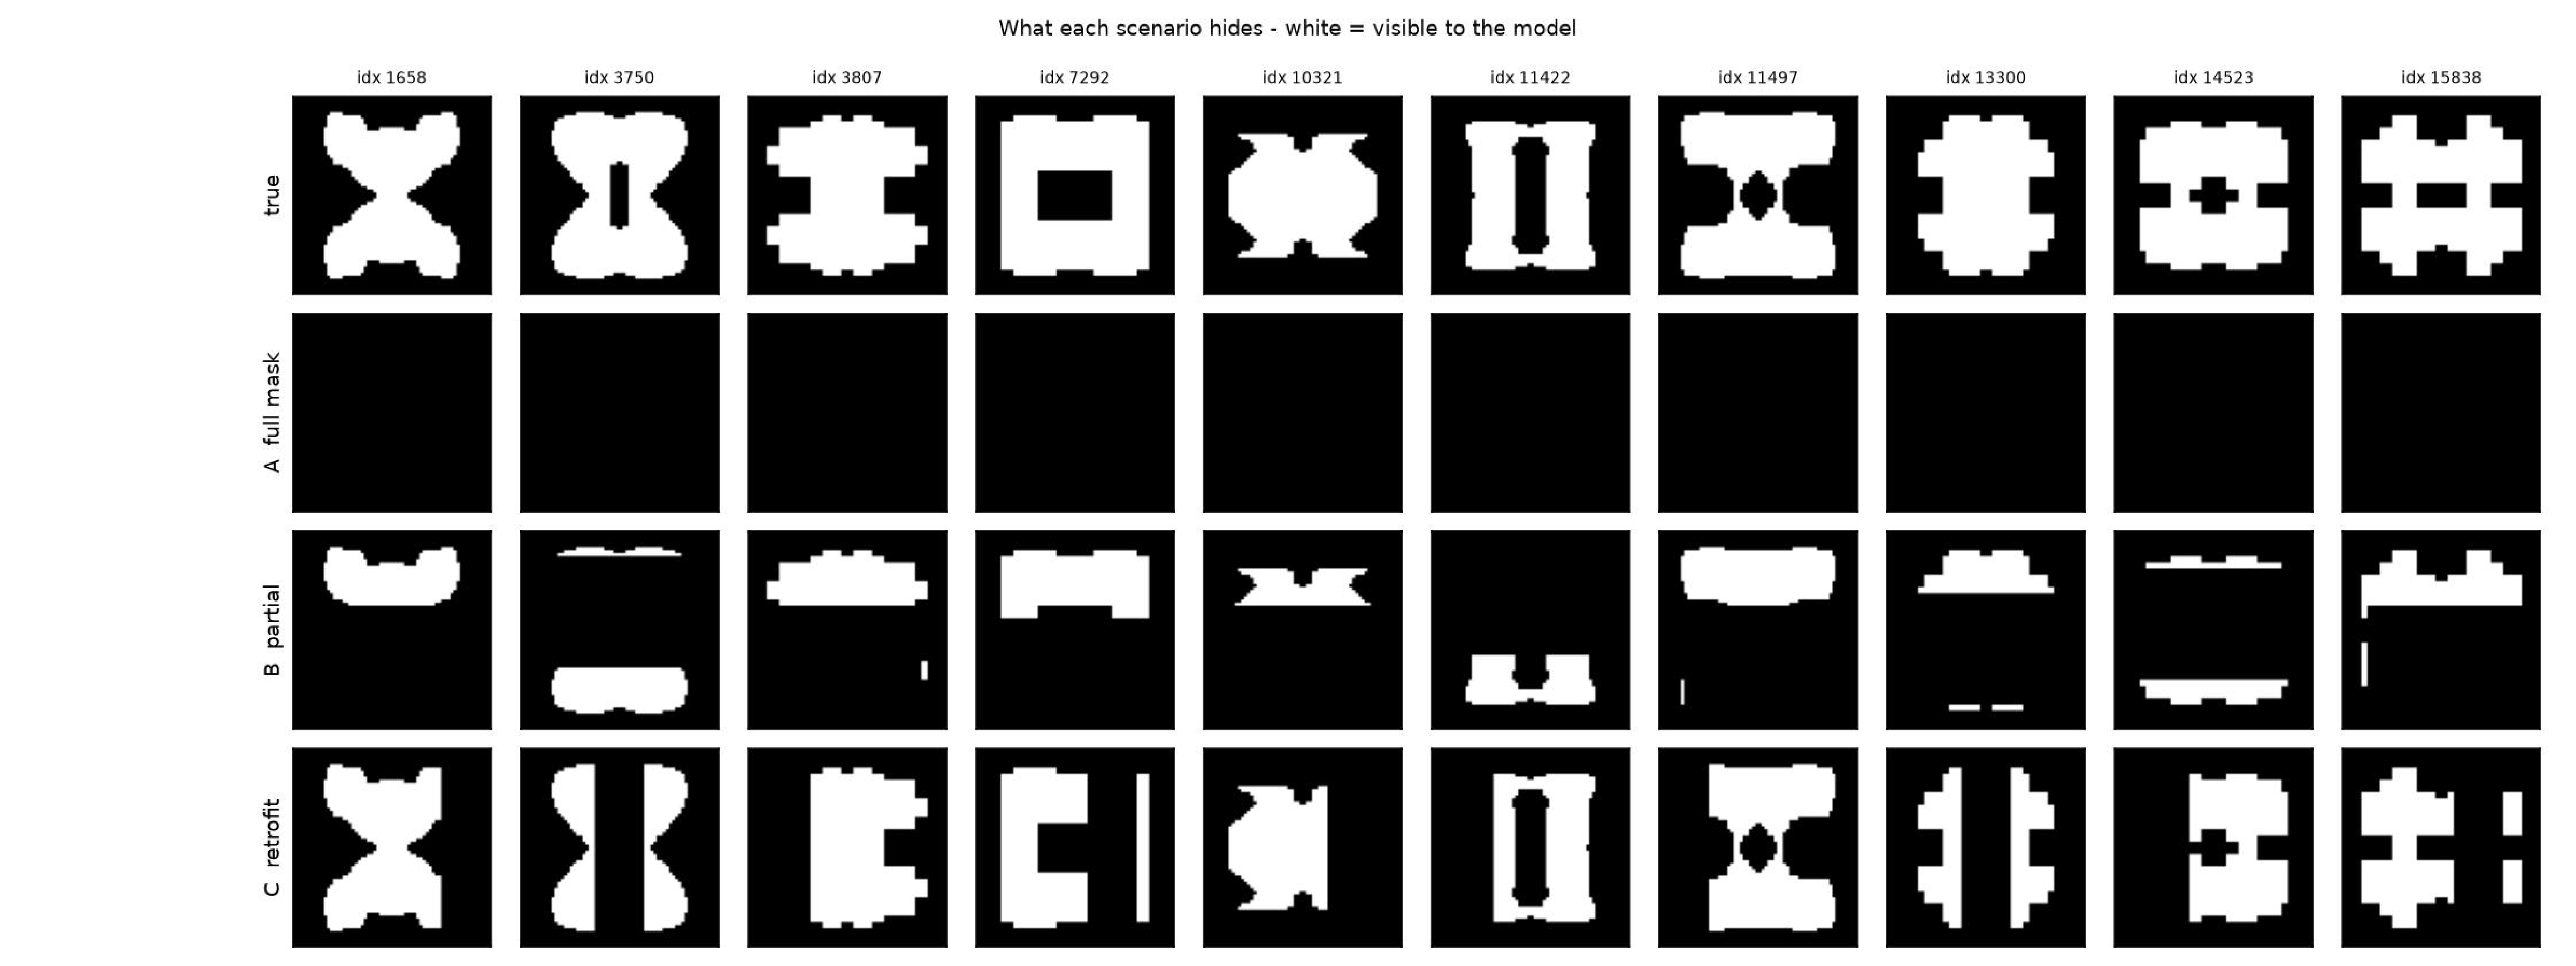
\includegraphics[width=\textwidth]{figs/masks.pdf}
\caption{What each regime reveals. White pixels are visible to the model; black pixels
must be generated. Row 2 hides the whole cell (spectrum only), row 3 hides half in two
bands, row 4 hides a quarter, leaving a vertical strip and a notch.}\label{fig:masks}
\end{figure}

The primary spectral metric is the per-sample mean absolute error divided by the
per-sample standard deviation of the target spectrum, which puts weak and strong
responses on one scale. For comparability we also report the unnormalised mean absolute
error (MAE) and the accumulated absolute error (AAE) over the full test split. Geometry
quality is reported as intersection-over-union and $F_1$ on the occupied class, together
with the predicted occupancy fraction; pixel accuracy is not used, because a decoder
that predicts empty cells would score well on it.

The per-sample error distribution has a heavy tail, so a mean-based verdict on a small
batch is unstable. We gate on a paired statistic instead: for each sample we compare the
error obtained with the true goal against the error obtained with a derangement of the
batch's goals, and report the fraction of samples on which the true goal wins. The
threshold is $0.75$, i.e.\ the true goal must be measurably better, not merely better
more often than not. A deranged goal is a stronger control than an absent one, because
it preserves the statistics of the condition while destroying its correspondence.

\subsection{Results}

Over three training seeds on the full held-out test split, the model reaches a mean
absolute error of $0.0524\pm0.0014$ and an accumulated error of $31.6\pm0.8$, against
$0.0801$ and $48.25$ for MetaDiT-S~\cite{metadit}. It does so with $11.6$M trainable
parameters against $37.2$M, a factor of $3.2$ (Table~\ref{tab:benchmark}).

\begin{table}[h]
\centering
\caption{Held-out test split, pure inverse design. Mean $\pm$ standard deviation over
three training seeds for our model; single released checkpoint for the baseline.}
\label{tab:benchmark}
\begin{tabular}{@{}lccc@{}}
\toprule
Model & Trainable parameters & MAE $\downarrow$ & AAE $\downarrow$ \\
\midrule
Ours (this work) & 11.57M & $\mathbf{0.0524 \pm 0.0014}$ & $\mathbf{31.6 \pm 0.8}$ \\
MetaDiT-S~\cite{metadit} (reproduced) & 37.20M & 0.0803 & 48.34 \\
\botrule
\end{tabular}
\end{table}

Table~\ref{tab:gates} reports the paired statistic for the three regimes on the
validation split, 512 samples per seed. The true goal beats a deranged goal on
$99.3\%$ of pure-inverse samples, $97.1\%$ of partial samples and $93.0\%$ of retrofit
samples, all above the $0.75$ threshold. The ordering follows the amount of information
supplied: the more of the answer that is given, the smaller the residual role of the
spectrum, and retrofit is the regime with the lowest error and the weakest gate.

\begin{table}[h]
\centering
\caption{Paired real-versus-deranged gate on the validation split ($n=512$ per seed,
three seeds).}\label{tab:gates}
\begin{tabular}{@{}lcccc@{}}
\toprule
Regime & Masked fraction & Parameters revealed & Spectrum error $\downarrow$ & Gate $\uparrow$ \\
\midrule
A pure inverse & 1.000 & none & $0.136 \pm 0.005$ & $\mathbf{0.993 \pm 0.003}$ \\
B partial & 0.492 & one & $0.102 \pm 0.003$ & $0.971 \pm 0.009$ \\
C retrofit & 0.250 & all three & $\mathbf{0.064 \pm 0.002}$ & $0.930 \pm 0.007$ \\
\botrule
\end{tabular}
\end{table}

The conditioning result is stronger than the 512-sample protocol above. On the hard
stratum, full occupancy mask with all three parameters unknown, the constrained model's seed-0
checkpoint gives a paired win rate of $99.35\%$ over 1{,}536 pooled evaluation samples,
against a decision threshold of $0.75$. The 1{,}536 are evaluation samples drawn under
three evaluation seeds, not independently trained models.

Occupancy $F_1$ on the occupied class is $0.88$ in the pure inverse regime and rises to
$0.92$ in retrofit. The predicted occupancy fraction is $0.43$ against a true $0.43$,
with a per-sample spread of the same order as the data's own, which rules out the
constant-output collapse that a pixel metric would miss.

Every generated design satisfies Eq.~\eqref{eq:sym} exactly, whereas an unconstrained
decoder on identical inputs produced asymmetric outputs. The constraint does not by
itself lower spectral error, and it leaves occupancy IoU essentially unchanged; its
benefit is that the output is admissible, which removes a class of failures that a
post-hoc symmetrisation would hide rather than prevent.

\clearpage
\begin{table}[h]
\centering
\caption{Controlled ablations on the canonical battery. Unless stated otherwise every arm
uses the \textbf{unconstrained} decoder, the full-resolution decoder without the symmetry
constraint; the last block isolates the decoder change against the constrained model that
Table~\ref{tab:benchmark} reports. Each block changes one factor against its own control.
Values are test-split MAE and validation-split scenario gate A, mean over three seeds.}
\label{tab:ablation}
\begin{tabular}{@{}llccc@{}}
\toprule
Factor & Variant & Trainable & MAE $\downarrow$ & Gate A $\uparrow$ \\
\midrule
model size & S0 tiny & 2.19M & $0.0564 \pm 0.0003$ & 0.997 \\
 & S1 small & 4.23M & $0.0542 \pm 0.0028$ & 0.992 \\
 & S2 slim & 8.14M & $0.0518 \pm 0.0009$ & 0.995 \\
 & base & 11.40M & $\mathbf{0.0490 \pm 0.0013}$ & $\mathbf{0.9967}$ \\
 & L1 wide & 19.90M & $0.0531 \pm 0.0036$ & 0.996 \\
\midrule
objective & JEPA & 11.40M & $\mathbf{0.0490 \pm 0.0013}$ & $\mathbf{0.9967}$ \\
 & supervised only & 11.40M & $0.0922 \pm 0.0195$ & 0.9792 \\
\midrule
train split & 60/20/20 & 11.40M & $0.0544 \pm 0.0013$ & 0.994 \\
 & 50/25/25 & 11.40M & $0.0552 \pm 0.0018$ & 0.991 \\
 & 40/40/20 & 11.40M & $0.0619 \pm 0.0006$ & 0.992 \\
\midrule
decoder & unconstrained (base) & 11.40M & $0.0490 \pm 0.0013$ & 0.9967 \\
 & constrained & 11.57M & $0.0524 \pm 0.0014$ & 0.993 \\
\botrule
\end{tabular}
\end{table}

\subsection{Qualitative comparison}

Figure~\ref{fig:designs} shows ten held-out test spectra decoded under all three regimes
together with the released baseline's output for the pure inverse regime. The baseline
produces coarser, stair-stepped shapes, a consequence of generating a $32\times32$
quadrant; our decoder produces the same symmetry at full $64\times64$ resolution. In
retrofit the visible pixels dominate and the difference narrows, as expected. Two
failure modes visible in the figure are worth naming: where the target admits several
designs the model returns a smooth compromise rather than one of the sharp alternatives,
and fine notches are rounded off, the qualitative counterpart of the conditional-mean
argument in Section~\ref{sec2}.

\begin{figure}[H]
\centering
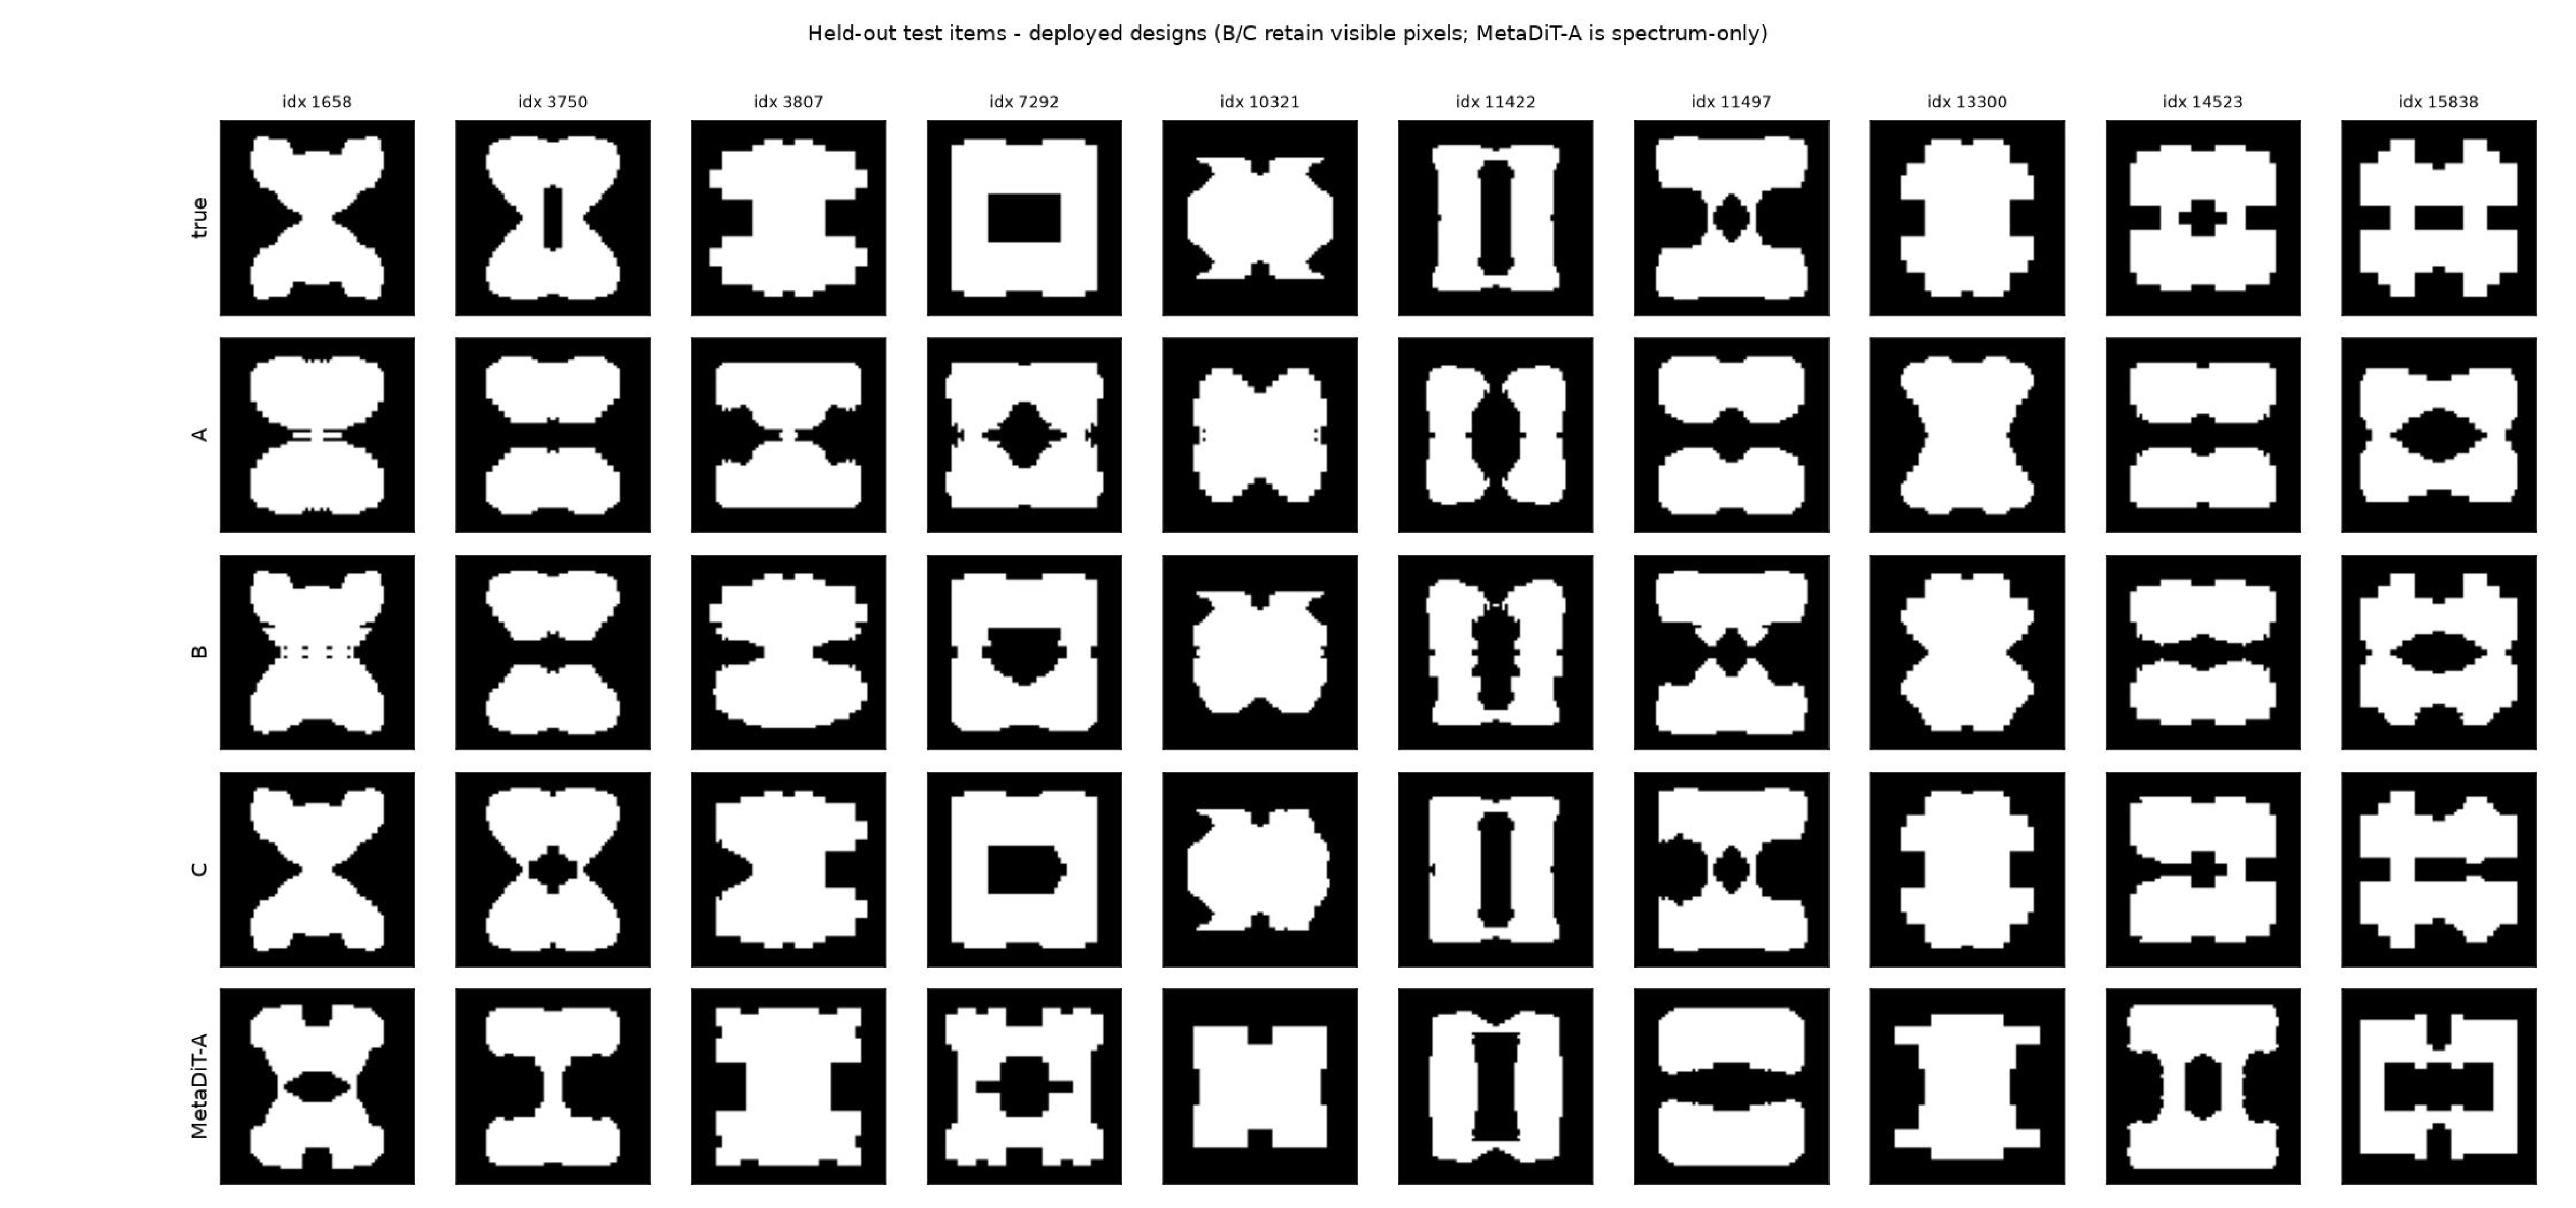
\includegraphics[width=\textwidth]{figs/designs.pdf}
\caption{Ten held-out test spectra. Rows: ground truth, pure inverse design, partial
design, retrofit, and the released baseline under the pure inverse regime. Each column
is one test sample; white denotes occupied material.}\label{fig:designs}
\end{figure}

Three limitations should be read alongside these numbers. Supplied scalar parameters are
not demonstrably used: the paired scalar-dependence statistics sit at $0.505$ and $0.529$
against a decision threshold of $0.75$, so the evidence supports strong spectral dependence
but not reliable parameter conditioning. The
benchmark is scored by the same frozen surrogate that supplies the physics term during
training, so it is a consistency measurement and not an independent physical validation; no
full-wave evaluation is reported here. And the model is deterministic: it returns one design
per target rather than a distribution over the admissible set, so the several-valid-answers
structure of the problem is acknowledged in the objective but not represented in the output.
A separate experiment in which guidance strength generated five candidates per target and
the measured spectra chose between them did not establish target-specific selection (10 of
18 targets, $p=0.81$), and we do not claim it.

\section{Conclusion and Future Scope}\label{sec5}

We have presented a factorised, goal-conditioned JEPA for metasurface inverse design
that treats masking of the geometry and of the parameters as independent operations,
conditions a latent-completion transformer on a frozen spectrum encoder through both
FiLM and attention tokens, and encodes the corpus's exact mirror symmetry in its
decoder. With $3.2\times$ fewer trainable parameters than the released baseline it
reaches a test-split MAE of $0.0524$ and passes the paired gate in all three regimes.

Three directions follow from the results. Output fidelity is the most immediate: the
decoder holds a small fraction of the parameters and the generated boundaries are
smoother than the recorded designs, which points at the output parameterisation rather
than the latent as the current bottleneck. Multi-modality is the second: the model is
deterministic, so for spectra with several admissible designs it returns an average of
them, and a stochastic or multi-hypothesis decoder is the natural remedy. External
validity is the third: every number here comes from one released corpus and one frozen
surrogate, and evaluation on independently acquired experimental data, together with
an independent full-wave solver~\cite{meep,maxim} rather than the surrogate that also
served as the training signal, would test the representation rather than the scorer.

\section*{Declarations}

\noindent\textbf{Funding.} This research received no external funding.

\vspace{0.3em}
\noindent\textbf{Conflict of Interest.} The authors declare that they have no conflict of interest.

\vspace{0.3em}
\noindent\textbf{Ethics Approval and Consent to Participate.} Not applicable. This study does not involve human participants, personal data, or animals.

\vspace{0.3em}
\noindent\textbf{Consent for Publication.} Not applicable.

\vspace{0.3em}
\noindent\textbf{Materials Availability.} All materials necessary to reproduce the experiments are described within the manuscript.

\vspace{0.3em}
\noindent\textbf{Author Contributions.} All authors contributed to the conception and design of the study and also, all authors reviewed and approved the final manuscript.

\vspace{0.3em}
\noindent\textbf{Data and Code Availability.} The source code, datasets, and supplementary materials supporting the findings of this study are maintained at
\url{https://github.com/tegga8/metasurface-jepa}.

\begingroup\small
\begin{thebibliography}{99}\bibitem{metadit} H.~Li \emph{et al.}, ``MetaDiT: enabling fine-grained constraints in
high-degree-of-freedom metasurface inverse design,'' in \emph{Proc. AAAI Conf. Artif.
Intell.}, vol.~40, no.~1, 2026. \href{https://doi.org/10.1609/aaai.v40i1.37025}{doi:10.1609/aaai.v40i1.37025}.

\bibitem{empowering} Z.~Li \emph{et al.}, ``Empowering metasurfaces with inverse design:
principles and applications,'' \emph{ACS Photonics}, vol.~9, no.~7, 
2022. \href{https://doi.org/10.1021/acsphotonics.1c01850}{doi:10.1021/acsphotonics.1c01850}.

\bibitem{roadmap} A.~I.~Kuznetsov \emph{et al.}, ``Roadmap for optical metasurfaces,''
\emph{ACS Photonics}, vol.~11, no.~3, 2024.
\href{https://doi.org/10.1021/acsphotonics.3c00457}{doi:10.1021/acsphotonics.3c00457}.

\bibitem{revisit} S.~So \emph{et al.}, ``Revisiting the design strategies for
metasurfaces: fundamental physics, optimization, and beyond,'' \emph{Adv. Mater.},
vol.~35, art.~2206399, 2023. \href{https://doi.org/10.1002/adma.202206399}{doi:10.1002/adma.202206399}.

\bibitem{genmodel} Z.~Liu, D.~Zhu, S.~P.~Rodrigues, K.-T.~Lee, and W.~Cai,
``Generative model for the inverse design of metasurfaces,'' \emph{Nano Lett.},
vol.~18, no.~10, 2018. \href{https://doi.org/10.1021/acs.nanolett.8b03171}{doi:10.1021/acs.nanolett.8b03171}.

\bibitem{tandem} D.~Liu, Y.~Tan, E.~Khoram, and Z.~Yu, ``Training deep neural networks
for the inverse design of nanophotonic structures,'' \emph{ACS Photonics}, vol.~5,
no.~4, 2018. \href{https://doi.org/10.1021/acsphotonics.7b01377}{doi:10.1021/acsphotonics.7b01377}.

\bibitem{structuralcolor} N.~B.~Roberts and M.~K.~Hedayati, ``A deep learning approach
to the forward prediction and inverse design of plasmonic metasurface structural
colour,'' \emph{Appl. Phys. Lett.}, vol.~119, art.~061101, 2021.
\href{https://doi.org/10.1063/5.0055733}{doi:10.1063/5.0055733}.

\bibitem{ailarge} M.~K.~Chen, L.~Zhu, C.-W.~Qiu, and D.~P.~Tsai, ``Artificial
intelligence in meta-optics,'' \emph{Chem. Rev.}, vol.~122, no.~18,
2022. \href{https://doi.org/10.1021/acs.chemrev.2c00012}{doi:10.1021/acs.chemrev.2c00012}.

\bibitem{deepmetasurfaces} ``Deep learning in metasurfaces: from automated design to
adaptive systems,'' \emph{Adv. Photonics}, vol.~7, no.~3, art.~034005, 2025.
\href{https://doi.org/10.1117/1.AP.7.3.034005}{doi:10.1117/1.AP.7.3.034005}.

\bibitem{largescale} C.~Kang \emph{et al.}, ``Large-scale photonic inverse design:
computational challenges and breakthroughs,'' \emph{Nanophotonics}, vol.~13, no.~20,
2024. \href{https://doi.org/10.1515/nanoph-2024-0127}{doi:10.1515/nanoph-2024-0127}.

\bibitem{vr} Z.~Li \emph{et al.}, ``Inverse design enables large-scale high-performance
meta-optics reshaping virtual reality,'' \emph{Nat. Commun.}, vol.~13, art.~2409, 2022.
\href{https://doi.org/10.1038/s41467-022-29973-3}{doi:10.1038/s41467-022-29973-3}.

\bibitem{moclip} S.~Rodionov, A.~Burguete-Lopez, M.~Makarenko, Q.~Wang, F.~Getman, and
A.~Fratalocchi, ``MOCLIP: a foundation model for large-scale nanophotonic inverse
design,'' \emph{Nat. Commun.}, vol.~17, art.~9902, 2026.
\href{https://doi.org/10.1038/s41467-026-76714-x}{doi:10.1038/s41467-026-76714-x}.

\bibitem{ijepa} M.~Assran \emph{et al.}, ``Self-supervised learning from images with a
joint-embedding predictive architecture,'' in \emph{Proc. IEEE/CVF Conf. Comput. Vis.
Pattern Recognit.}, 2023. \href{https://doi.org/10.1109/CVPR52729.2023.01513}{doi:10.1109/CVPR52729.2023.01513}.

\bibitem{mae} K.~He, X.~Chen, S.~Xie, Y.~Li, P.~Doll\'ar, and R.~Girshick, ``Masked
autoencoders are scalable vision learners,'' in \emph{Proc. IEEE/CVF Conf. Comput.
Vis. Pattern Recognit.}, 2022. \href{https://doi.org/10.1109/CVPR52688.2022.01553}{doi:10.1109/CVPR52688.2022.01553}.

\bibitem{film} E.~Perez, F.~Strub, H.~de~Vries, V.~Dumoulin, and A.~Courville, ``FiLM:
visual reasoning with a general conditioning layer,'' in \emph{Proc. AAAI Conf.
Artif. Intell.}, vol.~32, no.~1, 2018. \href{https://doi.org/10.1609/aaai.v32i1.11671}{doi:10.1609/aaai.v32i1.11671}.

\bibitem{meep} A.~F.~Oskooi, D.~Roundy, M.~Ibanescu, P.~Bermel, J.~D.~Joannopoulos, and
S.~G.~Johnson, ``Meep: a flexible free-software package for electromagnetic simulations
by the FDTD method,'' \emph{Comput. Phys. Commun.}, vol.~181, no.~3, 2010.
\href{https://doi.org/10.1016/j.cpc.2009.11.008}{doi:10.1016/j.cpc.2009.11.008}.

\bibitem{maxim} G.~Yoon and J.~Rho, ``MAXIM: metasurfaces-oriented electromagnetic wave
simulation software with intuitive graphical user interfaces,''
\emph{Comput. Phys. Commun.}, vol.~264, art.~107846, 2021.
\href{https://doi.org/10.1016/j.cpc.2021.107846}{doi:10.1016/j.cpc.2021.107846}.

\bibitem{dit} W.~Peebles and S.~Xie, ``Scalable diffusion models with transformers,'' in \emph{Proc. IEEE/CVF Int. Conf. Comput. Vis.}, 2023. \href{https://doi.org/10.1109/ICCV51070.2023.00387}{doi:10.1109/ICCV51070.2023.00387}.

\bibitem{vicreg} A.~Bardes, J.~Ponce, and Y.~LeCun, ``VICReg: variance-invariance-covariance regularization for self-supervised learning,'' in \emph{Int. Conf. Learn. Represent.}, 2022. \href{https://doi.org/10.48550/arXiv.2105.04906}{doi:10.48550/arXiv.2105.04906}.

\bibitem{vit} A.~Dosovitskiy \emph{et al.}, ``An image is worth 16x16 words: transformers for image recognition at scale,'' in \emph{Int. Conf. Learn. Represent.}, 2021. \href{https://doi.org/10.48550/arXiv.2010.11929}{doi:10.48550/arXiv.2010.11929}.

\bibitem{adamw} I.~Loshchilov and F.~Hutter, ``Decoupled weight decay regularization,'' in \emph{Int. Conf. Learn. Represent.}, 2019. \href{https://doi.org/10.48550/arXiv.1711.05101}{doi:10.48550/arXiv.1711.05101}.

\bibitem{ddpm} J.~Ho, A.~Jain, and P.~Abbeel, ``Denoising diffusion probabilistic models,'' in \emph{Adv. Neural Inf. Process. Syst.}, 2020. \href{https://doi.org/10.48550/arXiv.2006.11239}{doi:10.48550/arXiv.2006.11239}.

\end{thebibliography}
\endgroup

\end{document}
